\documentclass[
%draft%     uncomment to activate draft mode (see preamble/proofs)
]{article}   

% preamble -- do not rearrange order of \includes
%\include{classoptions}
%\include{pagesize}
%\include{packages}
%\include{encoding}         
%\include{fonts}
%\include{ToC}
%\include{contributor}
%\include{copyright}
%\include{bibtex}
%\include{environments}
%\include{sectionoptions}
%\include{headerfooter}
%\include{footnoteformat}
%\include{codesnipets}
%\include{proofs}
\usepackage{hyperref}
\hypersetup{
    colorlinks=true,
    linkcolor=blue,
    filecolor=magenta,      
    urlcolor=cyan,
    pdftitle={Overleaf Example},
    pdfpagemode=FullScreen,
    }
\usepackage{amsmath} % for align
\usepackage{subcaption}
\captionsetup{compatibility=false}
\usepackage{algorithm}% http://ctan.org/pkg/algorithms
\usepackage{algpseudocode}% http://ctan.org/pkg/algorithmicx
\usepackage[style=numeric,sorting=none]{biblatex}
\addbibresource{main.bib} %Import the bibliography file
\usepackage{tikz}
\usepackage{graphicx}
\usepackage[export]{adjustbox}
\usepackage{caption}
\usepackage{amssymb}
\usepackage{float}
% \usepackage{subfig}
\usepackage{placeins}
\usepackage{listings}
\lstset{
  basicstyle=\ttfamily,
  mathescape
}
%\usepackage{minted}
\usetikzlibrary{shapes}
\usetikzlibrary {positioning}
\usetikzlibrary{chains}
\usetikzlibrary{fit}
\usetikzlibrary{chains,shadows.blur}
\usepackage{geometry}
\usepackage{array}
\usepackage{hyperref}
\usepackage{indentfirst}
\usepackage{pdfpages}


\hypersetup{
    colorlinks=true,
    linkcolor=magenta,
    filecolor=cyan,      
    urlcolor=blue,
}
\graphicspath{ {./images/} }


\usepackage{listings}
\usepackage{xcolor}

\usepackage[autosize]{dot2texi}
\usepackage{tikz}
\usetikzlibrary{shapes,arrows}

\definecolor{codegreen}{rgb}{0,0.6,0}
\definecolor{codegray}{rgb}{0.5,0.5,0.5}
\definecolor{codepurple}{rgb}{0.58,0,0.82}
\definecolor{backcolour}{rgb}{0.95,0.95,0.92}
\usepackage{tcolorbox}

\newtcolorbox{note}[1]{colback=red!5!white,colframe=red!75!black,fonttitle=\bfseries,title=#1}


\newtcolorbox{definition}[1]{colback=blue!5!white,colframe=blue!75!black,fonttitle=\bfseries,title=#1}


\lstdefinestyle{mystyle}{
    % backgroundcolor=\color{backcolour},   
    commentstyle=\color{codegreen},
    keywordstyle=\color{magenta},
    numberstyle=\tiny\color{codegray},
    stringstyle=\color{codepurple},
    basicstyle=\ttfamily\footnotesize,
    breakatwhitespace=false,         
    breaklines=true,                 
    captionpos=b,                    
    keepspaces=true,                 
    numbers=left,                    
    numbersep=5pt,                  
    showspaces=false,                
    showstringspaces=false,
    showtabs=false,                  
    tabsize=2
}

\newtcolorbox{proof}[1]{colback=white,colframe=gray,fonttitle=\bfseries,title=#1}

\newtcolorbox{question}[1]{colback=white,colframe=gray,fonttitle=\bfseries,title=#1}


% \usepackage[margin=1in]{geometry} 
% \usepackage[T1]{fontenc}
% \usepackage{lmodern}
% \usepackage{mathtools,amssymb}

% \usepackage{graphicx}
% \usepackage{color}
% \usepackage{tikz}
% \usetikzlibrary{positioning}
% \usepackage{microtype}
% \usepackage{hyperref}

% \newcommand{\TODO}[1]{{\color{red}\textit{todo:} #1}}

% % problem and problempart environments.
% % \begin{problem}
% %     ...
% %     \begin{problempart}
% %         ...
% %     \end{problempart}
% %     \begin{problempart}
% %         ...
% %     \end{problempart}
% % \end{problem}
% \newcounter{problem}
% \providecommand*{\problemname}{Problem}
% \renewcommand{\theproblem}{\arabic{problem}}
% \newcounter{problempart}[problem]
% \providecommand*{\problempartname}{Problem}
% \renewcommand{\theproblempart}{\arabic{problem}\alph{problempart}}
% \newenvironment{problem}[1][Problem]{\begin{trivlist}%
% \item[\hskip\labelsep {\bfseries #1}~{\bfseries \refstepcounter{problem}\arabic{problem}\label{prob:\theproblem}.}]%
% \addcontentsline{toc}{section}{\protect\numberline{\theproblem} Problem \theproblem}}%
% {\end{trivlist}}
% \newenvironment{problempart}[1][Part]{\begin{trivlist}%
% \item[\hskip\labelsep {\bfseries #1}~{\bfseries \refstepcounter{problempart}\alph{problempart}\label{prob:\theproblempart}.}]%
% \addcontentsline{toc}{subsection}{\protect\numberline{\alph{problempart}} Part \alph{problempart}}}%
% {\end{trivlist}}

% \newcommand{\outs}{\ensuremath{\textsc{out}}}
% \newcommand{\ins}{\ensuremath{\textsc{in}}}
% \newcommand{\exit}{\ensuremath{\textsc{exit}}}
% \newcommand{\entry}{\ensuremath{\textsc{entry}}}



\usepackage{lmodern}
\usepackage{enumitem}
\usepackage{mathtools,amssymb}

\usepackage{graphicx}
\usepackage{color}
\usepackage{tikz}
\usetikzlibrary{positioning}
\usepackage{microtype}
% \usepackage[colorlinks]{hyperref}

\newcommand{\TODO}[1]{{\color{red}\textit{todo:} #1}}

\tikzset{
    placeholder/.style={text width=6em, font=\mathstrut},
    bb/.style={draw, align=center, placeholder},
    every label/.style={font=\small}}


\newcounter{problem}
\providecommand*{\problemname}{Problem}
\renewcommand{\theproblem}{\arabic{problem}}
\newcounter{problempart}[problem]
\providecommand*{\problempartname}{Problem}
\renewcommand{\theproblempart}{\arabic{problem}\alph{problempart}}
\newenvironment{problem}[1][Problem]{\begin{trivlist}%
\item[\hskip\labelsep {\bfseries #1}~{\bfseries \refstepcounter{problem}\arabic{problem}\label{prob:\theproblem}.}]%
\addcontentsline{toc}{subsection}{\protect\numberline{\theproblem} Problem \theproblem}}%
{\end{trivlist}}
\newenvironment{problempart}[1][Part]{\begin{trivlist}%
\item[\hskip\labelsep {\bfseries #1}~{\bfseries \refstepcounter{problempart}\alph{problempart}\label{prob:\theproblempart}.}]%
\addcontentsline{toc}{subsubsection}{\protect\numberline{\alph{problempart}} Part \alph{problempart}}}%
{\end{trivlist}}

\newcommand{\outs}{\ensuremath{\textsc{out}}}
\newcommand{\ins}{\ensuremath{\textsc{in}}}
\newcommand{\exit}{\ensuremath{\textsc{exit}}}
\newcommand{\entry}{\ensuremath{\textsc{entry}}}

\tikzset{
    placeholder/.style={text width=6em, font=\mathstrut},
    bb/.style={draw, align=center, placeholder},
    every label/.style={font=\small}}


% \lstset{style=mystyle}


%   \lstset{ %
%     language=Octave,                % the language of the code
%     basicstyle=\footnotesize,           % the size of the fonts that are used for the code
%     numbers=left,                   % where to put the line-numbers
%     numberstyle=\tiny\color{gray},  % the style that is used for the line-numbers
%     stepnumber=2,                   % the step between two line-numbers. If it's 1, each line 
%                                     % will be numbered
%     numbersep=5pt,                  % how far the line-numbers are from the code
%     backgroundcolor=\color{white},      % choose the background color. You must add \usepackage{color}
%     showspaces=false,               % show spaces adding particular underscores
%     showstringspaces=false,         % underline spaces within strings
%     showtabs=false,                 % show tabs within strings adding particular underscores
%     frame=single,                   % adds a frame around the code
%     rulecolor=\color{black},        % if not set, the frame-color may be changed on line-breaks within not-black text (e.g. commens (green here))
%     tabsize=2,                      % sets default tabsize to 2 spaces
%     captionpos=b,                   % sets the caption-position to bottom
%     breaklines=true,                % sets automatic line breaking
%     breakatwhitespace=false,        % sets if automatic breaks should only happen at whitespace
%     title=\lstname,                 % show the filename of files included with \lstinputlisting;
%                                     % also try caption instead of title
%     keywordstyle=\color{blue},          % keyword style
%     commentstyle=\color{dkgreen},       % comment style
%     stringstyle=\color{mauve},         % string literal style
%     escapeinside={\%*}{*)},            % if you want to add LaTeX within your code
%     morekeywords={*,...}               % if you want to add more keywords to the set
% }


% define issue details
\title{Compiler Optimization Notes}
\newcommand\thejournalsubtitle{Notes for the Compiler Optimization Techniques}
\newcommand\thevolume{}
\newcommand\theseason{May}
\newcommand\theyear{2022}
\newcommand\theissue{\thejournal \ \thevolume \ (\theyear)} 

\newcommand\generaleditor{}
\newcommand\associateeditor{}
\sloppy
\newcommand\thewebsite{https://github.com/liusy58/CompilerNotes}

\begin{document}
\sloppy                         % preferences more space between words over overrunning margins
\lefthyphenmin=3                % suppresses hyphenation after only 1 or 2 characters
                                % NB: You will need to repeat \lefthyphenmin in the text if you use \selectlanguage
%\include{editorialboard}
%\include{titlepage}
%\include{colofon}
\pagenumbering{roman}           
%\tableofcontents  
\thispagestyle{empty}

\maketitle
\tableofcontents

% \include{essays/preface}
\pagenumbering{arabic}


% \input{Foundations-of-Dataflow.tex}
% \input{More Examples of Data Flow Analysis}


\input{LocalOptimizations.tex}
\input{IntroToDFA.tex}
\input{Reaching Definitions.tex}
\input{Live Variabl Analysis.tex}
\input{Available Expressions Analysis.tex}
\input{Constant Propagation.tex}
\input{Foundations of Data Flow Analysis.tex}
\input{Introduction To SSA}
\input{SSA-Style Optimizations.tex}
\input{LLVMProj.tex}
\input{LICM.tex}
\input{SR.tex}
\input{PRE.tex}
\input{LCM.tex}
\input{AnotherLCM.tex}
\input{RA.tex}
\input{PA.tex}
\input{RegAlloc.tex}
\input{LS.tex}
\input{SoftwarePipe.tex}
\input{Dynamic Code Optimization.tex}
\input{DSL.tex}
\input{MHO.tex}
\newpage

\section{Data Prefetching}
\subsection{Compiler-Based Prefetching for Recursive Data Structures\cite{luk1996compiler}}

Recursive Data Structures (RDSs) include familiar objects
such as linked lists, trees, graphs, etc., where individual nodes
are dynamically allocated from the heap, and nodes are linked
together through pointers to form the overall structure. For
our purposes, "recursive data structures" can be broadly interpreted to include most pointer-linked data structures (e.g.,
mutually-recursive data structures, or even a graph of heterogeneous objects). From a memory performance perspective, these
pointer-based data structures are expected to be an important
concern for the following reasons. For an application to suffer a large memory penalty due to data replacement misses, it
typically must have a large data set relative to the cache size.
Aside from multi-dimensional arrays, recursive data structures
are one of the most common and convenient methods of building
large data structures (e.g, B-trees in database applications, octrees in graphics applications, etc.). As we traverse a large RDS,
we may potentially visit enough intervening nodes to displace a
given node from the cache before it is revisited; hence temporal
locality may be poor. Finally, in contrast with arrays, where
consecutive elements are at contiguous addresses and therefore
stride-one accesses can exploit long cache lines, there is little inherent spatial locality between consecutively-accessed nodes in
an RDS since they are dynamically allocated from the heap and
can have arbitrary addresses. Therefore, techniques for coping
with the latency of accessing these pointer-based data structures
are essential.



\subsubsection{Challenges in Prefetching RDSs }


Any software-controlled prefetching scheme can be viewed as having two major phases. First, an analysis phase predicts which dynamic memory references are likely to suffer caches misses, and
hence should be prefetched. Second, a scheduling phase attempts
to insert prefetches sufficiently far in advance such that latency is
effectively hidden, while introducing minimal runtime overhead.
For array-based applications, the compiler can use locality analysis to predict which dynamic references to prefetch, and loop
splitting and software pipelining to schedule prefetches.

A fundamental difference between array references and pointer
dereferences is the way addresses are generated. The address of
an array reference \texttt{A[i]} can always be computed once a value of
i is chosen. In contrast, the address of a pointer dereference *p
is unknown unless the value stored in \texttt{p} is read. This difference
makes both the analysis and scheduling phases significantly more
challenging for RDSs than for arrays.


\subsubsection{Analysis}
To illustrate the difficulty of analyzing data locality in RDSs,
consider the code in Figure \ref{fig:p247}(a), where we are traversing n different linked lists. In one extreme, the nodes may be entirely
disjoint (as illustrated in Figure \ref{fig:p247}(b)), in which ease we would
want to prefetch every list node. Another possibility might be
that each list shares a long common "tail" starting with the second list node (as illustrated in Figure \ref{fig:p247}(c)). In this latter case,
there would be significant temporal locality (assuming the cache
is large enough to contain the common tail), and ideally we would
only want to prefetch the nodes in the common tail during the
first list traversal (i.e. when \texttt{i=1}). Unfortunately, despite the
significant progress that has been made recently in pointer analysis techniques for heap-allocated objects [6, 8, 10], compilers are
still not sophisticated enough to differentiate these two cases automatically. In general, analyzing the addresses of heap-allocated
objects is a very difficult problem for the compiler.




\begin{figure}[H]
    \centering
    \includegraphics[width=0.6\textwidth]{p247.png}
    \caption{Example of list traversals, both with and without temporal data locality. }
    \label{fig:p247}
\end{figure}



\subsubsection{Scheduling}

Our ability to schedule prefetches for an RDS is also constrained
by the fact that nodes are linked together through pointers. For
example, consider the case shown in Figure \ref{fig:p248}(a), where assuming
that three nodes worth of computation is needed to hide the
latency, we would like to initiate a prefetch for node $n_{i+3}$  while
we are visiting node $n_i$ The problem is that to compute the
address of node $n_{i+3}$ , we must first dereference a pointer in node
$n_{i+2}$ , and to do that, we must first dereference a pointer in node
$n_{i+1}$  etc. As a result, one cannot prefetch (or fetch) a future
node until all nodes between it and the current node have been
fetched. However, the very act of touching these intermediate
nodes means that we cannot tolerate the latency of fetching more
than one node ahead. For example, the prefetching code shown
in Figure \ref{fig:p248}(b) will not hide any more latency than the code in
Figure \ref{fig:p248}(c).1 In fact, the code in Figure \ref{fig:p248}(c) is likely to run faster
since it has less instruction overhead. This example illustrates
what we refer to as the pointer-chasing problem.

Since scheduling RDS prefetches is such a difficult problem, we
make it the primary focus of this paper. Improvements in analysis tend to reduce prefetching overhead by eliminating unnecessary prefetches. However, without sufficient scheduling techniques, there will be no upside to prefetching and hence reducing
overhead will be irrelevant. Fortunately, as we discuss in the
next subsection, there are techniques for scheduling prefetches
that avoid the pointer-chasing problem.



\begin{figure}[H]
    \centering
    \includegraphics[width=0.6\textwidth]{p248.png}
    \caption{Illustration of the pointer-chasing problem.  }
    \label{fig:p248}
\end{figure}


\subsubsection{Greedy Prefetching}

In a k-ary RDS, each node contains k pointers to other nodes.
Greedy prefetching exploits the fact that when $k > 1$, only one
of these $k$ pointers can be immediately followed by control flow
as the next node in the traversal. Hence the remaining $k - 1$
pointers serve as natural jump-pointers, and can be prefetched
immediately upon first visiting a node. Although none of these
jump-pointers may actually point to $n_{i+d}$ , hopefully each of them
points to $n_{i+d^{\prime}}$ , for some $d^{\prime}  > 0$. If $d^{\prime} < d$, then the latency may
be partially hidden; if  > d, then we expect the latency to be
fully hidden, provided that the node is not displaced from the
cache before it is referenced (which may occur if $d^{\prime} >> d$).

To illustrate how greedy prefetching works, consider the preorder
traversal of a binary tree (i.e. $k = 2$), where Figure \ref{fig:p249}(a)
shows the code with greedy prefetching added. Assuming that
the computation in \texttt{process()} takes half as long as the cache
miss latency, we would want to prefetch two nodes ahead (i.e.
$d = 2$) to fully hide the latency. Figure \ref{fig:p249}(b) shows the caching
behavior of each node. We obviously suffer a full cache miss at
the root node (node 1), since there was no opportunity to fetch
it ahead of time. However, we would only suffer half of the miss
penalty ($\frac{L}{2}$) when we visit node 2, and no miss penalty when
we eventually visit node 3 (since the time to visit the subtree
rooted at node 2 is greater than $L$). In this example, the latency
is fully hidden for roughly half of the nodes, and reduced by
50\% for the other half (minus the root node). If we generalize
this example to a k-ary tree, we would expect the fraction of
nodes where latency is fully hidden to be roughly $\frac{k-1}{k}$(assuming
that prefetched nodes are generally not displaced from the cache
before they are referenced). Hence a larger value of $k$ is likely
to improve the performance of greedy prefetching, since more
natural jump-pointers are available.


\begin{figure}[H]
    \centering
    \includegraphics[width=0.6\textwidth]{p249.png}
    \caption{Illustration of greedy prefetching.  }
    \label{fig:p249}
\end{figure}


Greedy prefetching offers the following advantages:
(i) it has
low runtime overhead, since no additional storage or computation is needed to construct the natural jump-pointers;
(ii) it is
applicable to a wide variety of RDSs, regardless of how they are
accessed or whether their structure is modified frequently; and
(iii) it is relatively straightforward to implement in a compiler. The main disadvantage of greedy prefetching is that it does not offer precise control over the prefetching
distance, which is the motivation for our next algorithm.



\input{Parallelism and Dependence Theory.tex}
\input{TLS.tex}
\input{PGO.tex}
\input{Concurrent.tex}
\input{CPP.tex}
\input{C++11MemoryModel.tex}
\newpage

\section{Dependence Analysis}



\subsection{Dependence in Loops}

If there are no dependences in a loop, we can parallelize it because none of the 
iterations interfere with each other. Loop dependence is also useful in other loop optimizations, such
as loop interchange, loop fusion, etc.

In this section, we should answer the following two questions:

\begin{itemize}
\item How do we represent dependences in loops?
\item How do we determine if there are dependences?
\end{itemize}    


\subsubsection{Representing dependences}

Iteration space graphs is a good start. Here we give steps for creating 
iteration space graphs:

\begin{itemize}
    \item Step 1: Create nodes, 1 for each iteration
    \item Step 2: Determine which array elements are read and
    written in each iteration
    \item Step 3: Draw arrows to represent dependences
\end{itemize}    
    

\begin{figure}[H]
    \centering
    \begin{subfigure}{0.6\textwidth}
    \centering
        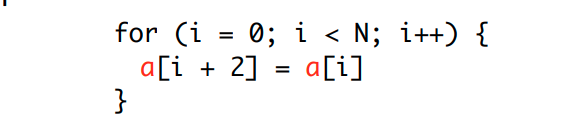
\includegraphics[width=\textwidth]{p253.png}
        \caption{Source code.}
        \label{fig:p253}
    \end{subfigure}
    \begin{subfigure}{0.6\textwidth}
    \centering
        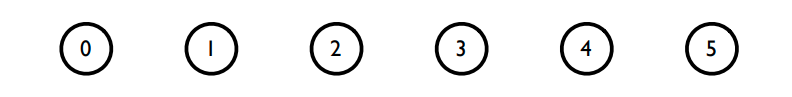
\includegraphics[width=\textwidth]{p250.png}
        \caption{Step 1: Create nodes, 1 for each iteration}
        \label{fig:p250}
    \end{subfigure}
    \begin{subfigure}{0.6\textwidth}
        \centering
            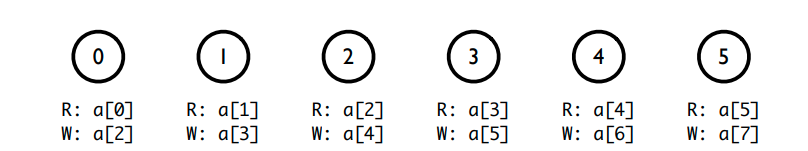
\includegraphics[width=\textwidth]{p251.png}
            \caption{Step 2: Determine which array elements are read and
            written in each iteration}
            \label{fig:p251}
        \end{subfigure}
    \begin{subfigure}{0.6\textwidth}
            \centering
                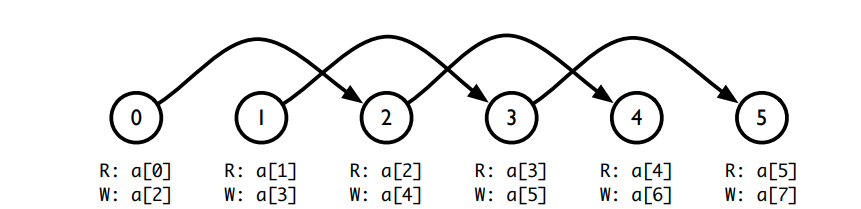
\includegraphics[width=\textwidth]{p252.png}
                \caption{Step 3: Draw arrows to represent dependences}
                \label{fig:p252}
    \end{subfigure}    
    \caption{A 1-D exmaple to illustrate Iteration space graphs.}
       \label{fig:p253}
\end{figure}



\begin{figure}[H]
    \centering
    \begin{subfigure}{0.5\textwidth}
    \centering
        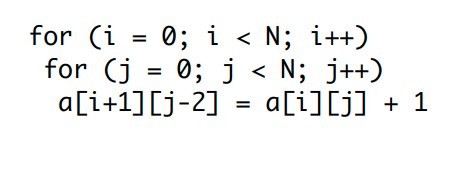
\includegraphics[width=\textwidth]{p255.png}
        \caption{Source code.}
        \label{fig:p255}
    \end{subfigure}
    \begin{subfigure}{0.5\textwidth}
    \centering
        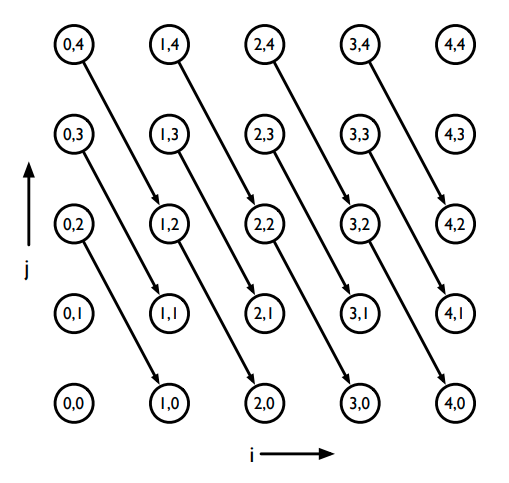
\includegraphics[width=\textwidth]{p254.png}
        \caption{Iteration space graphs for the source code.}
        \label{fig:p254}
    \end{subfigure}
  
    \caption{A 2-D exmaple to illustrate Iteration space graphs.}
       \label{fig:p254-5}
\end{figure}


But there is a crucial problem faced by iteration space graph: 
Iteration space graphs are potentially infinite representations!

Compiler researchers have devised compressed representations of dependences, such 
as distance vectors and direction vectors.

\subsubsection{Distance vector}

Distance vectors captures the “shape” of dependences,
but not the particular source and sink. Represent each dependence arrow in an iteration space
graph as a vector.

Distance vectors for Figure \ref{fig:p252} is $ (2) $. 
Distance vectors for Figure \ref{fig:p254} is $ (1,-2) $.


A more complex example is shown in \label{fig:p256-7}.
There are 2 distance vectors : $(1,-2), (2,0)$.




\begin{figure}[H]
    \centering
    \begin{subfigure}{0.5\textwidth}
    \centering
        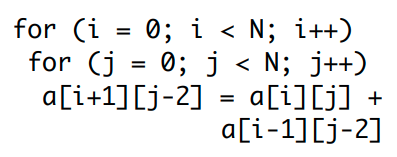
\includegraphics[width=\textwidth]{p256.png}
        \caption{Source code.}
        \label{fig:p256}
    \end{subfigure}
    \begin{subfigure}{0.5\textwidth}
    \centering
        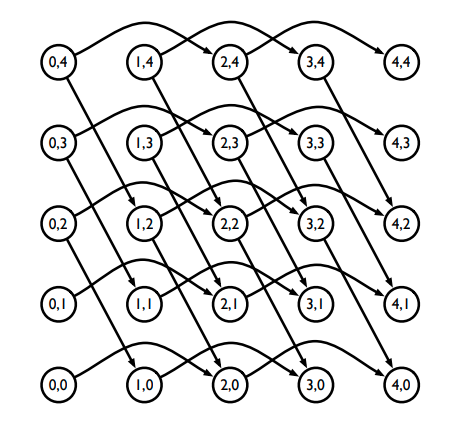
\includegraphics[width=\textwidth]{p257.png}
        \caption{Iteration space graphs for the source code.}
        \label{fig:p257}
    \end{subfigure}
  
    \caption{A 2-D exmaple to illustrate Iteration space graphs.}
       \label{fig:p256-7}
\end{figure}


But distance vectors can't always summarize as easily. Consider the example in
\ref{fig:p258}, distance vectors for this code are $(1), (2), (3), (4) ...$



\begin{figure}[H]
    \centering
    \begin{subfigure}{0.5\textwidth}
    \centering
        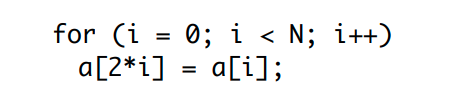
\includegraphics[width=\textwidth]{p258.png}
        \caption{Source code.}
        \label{fig:p258}
    \end{subfigure}
    \begin{subfigure}{0.7\textwidth}
    \centering
        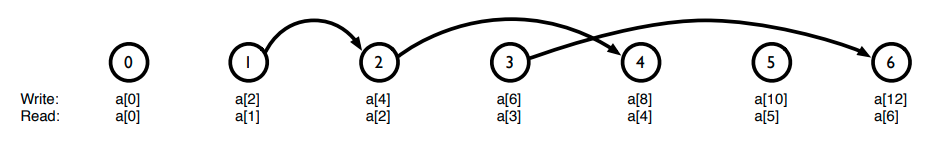
\includegraphics[width=\textwidth]{p259.png}
        \caption{Iteration space graphs for the source code.}
        \label{fig:p259}
    \end{subfigure}
  
    \caption{A 2-D exmaple to illustrate Iteration space graphs.}
       \label{fig:p258-9}
\end{figure}

From distance vector, we have information about the length of each vector,
but not about the source of each vector. What happens if we try to reconstruct the iteration space graph?



\begin{figure}[H]
    \centering
    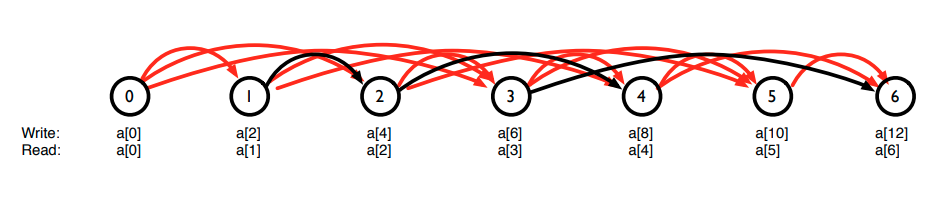
\includegraphics[width=0.8\textwidth]{p260.png}
    \caption{reconstruct the iteration
    space graph from distance vector for \ref{fig:p258}}
    \label{fig:p260}
\end{figure}


\subsection{Direction vectors}

The whole point of distance vectors is that we want to be able to
succinctly capture the dependences in a loop nest and summarize distance vectors, and save only the direction the
dependence was in.


For example, distance vector $(2,-1)$, the corresponding direction vector is $(+,-)$.
Also, distance vector $(0,1)$, the corresponding direction vector is $(0,+)$.

Direction vectors lose a lot of information, but do capture
some useful information, such as whether there is a dependence (anything other than a
$0$ means there is a dependence). 
Many times, the only information we need to determine if
an optimization (e.g. loop paralelization, loop iterchange) is legal is captured by direction vectors. 



If there is a non-zero entry for a loop dimension, that
means that there is a loop carried dependence over that
dimension. If an entry is zero, then that loop can be parallelized!





\subsubsection{Loop-carried dependence}

Loop carried dependence is a dependence that crosses loop iterations.

If there is a  loop carried dependence, then that loop cannot
be parallelized. 


\subsection{Data Dependence Tests}


\subsubsection{GCD}



\begin{figure}[H]
    \centering
    
\includegraphics[width=0.6\textwidth]{p261.png}
    \caption{}
    \label{fig:p261}
\end{figure}

Consider the loop nest in \ref{fig:p261} , A dependence exists if there exist an integer $i$ and an $i^\prime$ such
that:
\begin{itemize}
    \item  $f(i) = g(i^\prime)$
    \item  $0 \leq i, i^\prime < N$
    \item  If $i < i^\prime$, write happens before read (flow dependence)
    \item  If $i > i^\prime$, write happens after read (anti dependence)
\end{itemize}




An equation $a_1 \times i + a_2 \times i^\prime = a_3$ has a solution iff $gcd(a_1, a_2)$
evenly divides $a_3$

For example,
\begin{itemize}
    \item $15 \times i + 6 \times j - 9 \times k = 12$ has a solution (gcd = 3)
    \item $2 \times i + 7 \times j = 3$ has a solution (gcd = 1)
    \item $9 \times i + 6 \times j = 10$ has no solution (gcd = 3)
\end{itemize}



Unfortunately, most loops have gcd(a, b) = 1, which divides
everything. Also, If $f(i) = g(i^\prime)$, there might be a dependence, 
but might not.

\newpage

\section{Alias Analysis\footnote{based on \cite{ShengHsi98:online}}}

The purpose of alias analysis is to determine all possible ways a program may access some given
memory locations. A set of pointers are said to be in an alias group if they all point to the same
memory locations.  Alias analysis is very important in compiler theory. Some of its most notable applications
include code optimization and security. Compiler level optimization needs pointer aliasing information to perform dead code elimination (removing code that does not affect the program’s
result), redundant load/store instruction elimination, instruction scheduling (rearranging instructions) and more. Program security enforcement at compiler level uses alias analysis to help detect
memory leaks and memory related security holes.


\subsection{Clients of Alias Analysis}

Alias Analysis is not an optimization in itself, i.e., once alias analysis is run, it does not make the
program run faster. A Program transformation called Client need to query alias information from
alias analysis to create an optimized version of the program. Also, there are some other analysis
that don’t alter the code, but make use of alias analysis to compute better dataflow information
which can be used by other transformation. Examples of transformation clients include, Automated
bug correction, Parallelization, Common subexpression elimination. Examples of analysis clients
include, Slicing, Shape analysis.

\subsection{Types of Alias analysis}

There are many varieties of alias analysis. They are often categorized by properties such as
field-sensitivity, inter-procedural v.s. intra-procedural, context-sensitivity and flow-sensitivity.


\subsubsection{Field-Sensitivity}

Field-sensitivity is the strategy that governs the way alias analysis models fields in built-in or
user defined data structures. There are three approaches to field-sensitivity – field-sensitive,
field-insensitive and field-based. Consider the following code:

\lstinline[language=C]|struct { int a , b ; } x , y ;|



\begin{itemize}
\item Field-sensitive approach models each field of each struct variable, hence creating four nodes
(we use node to denote a pointer, variable or memory location)  \lstinline[language=C]|x.a, x.b, y.a and y.b.|

\item Field-insensitive approach models each struct variable, but does not model their fields. This
example is modeled by two nodes  \lstinline[language=C]|x.* and y.*.|

\item Field-based approach models each field without modeling the struct variables. This example
is modeled by two nodes  \lstinline[language=C]|*.a and *.b.|


\end{itemize}    

The same principle applies when dealing with arrays. Consider a C integer array int \lstinline[language=C]|a[10]|
Field-insensitive approach models this with only one node: a[*], while field-sensitive approach
creates ten nodes: \lstinline[language=C]|a[0], a[1], ..., a[10].|
Clearly a field-sensitive approach provides a more fine grained model and hence better precision. However, the number of nodes increases rapidly when there are nested structs and/or
arrays.


\subsubsection{Intra-Procedural v.s. Inter-Procedural}

An intra-procedural alias analysis analyzes the bodies of each functions. It does not consider
how each function interact with other functions. Specifically, intra-procedural alias analysis does
not handle pointer parameter passing or functions that return pointers. On the contrary, interprocedural alias analysis deals with the pointer behaviors due to function calls.

A pseudo-code where pointer parameter passing is involved:

\begin{lstlisting}[language=C]
void fn1(int * p) { p = ...}
void fn2 () { int * q ; fn1 ( q ) ; }
\end{lstlisting}


A pseudo-code where function is returning pointers:
\begin{lstlisting}[language=C]
    int * id ( int * p ) { return p ; }
    void fn () {
        int * q ;
        q = id ( q ) ;
    }
\end{lstlisting}

Intra-procedural is less expansive to perform, but has lower precision. It is often easier to
implement an intra-procedural alias analysis before extending to inter-procedural alias analysis.
Intra/inter-procedural property is highly related to context-sensitivity since a context-sensitive
analysis has to be an inter-procedural analysis.


\subsubsection{Context-Sensitivity}
Context-sensitivity governs how function calls are analyzed. This property yields two types of
alias analyses ? context-sensitive and context-insensitive alias analyses. Context-sensitive analysis
considers the calling context (caller) when analyzing the target of a function call (callee). Consider
the following code:


\begin{lstlisting}[language=C]
     int a , b ;
     int * x ;
    
     void f ( void ) { * x ++; }
    
     void main () {
        x = & a ;
        f () ;
        
        x = & b ;
        f () ;
     }
\end{lstlisting}



In this code, function-f is called twice. It increases the value of variable-a the first time it
was called, and increases the value of variable-b the second time it was called. A context-sensitive
alias analyzer needs to have a way to create an abstract description for function-f so that every
time it is called, the analyzer can apply the calling context to the abstract description.
Context-sensitive provides a finer grain model of the static code hence results in higher precision. However, it increases the complexity of the analysis.





\subsubsection{Flow-Sensitivity}


Flow-sensitivity is the principle that governs wether or not an analysis takes the order of code
into account. There are flow-sensitive and flow-insensitive analyses.
A flow-insensitive analysis produces one set of alias result for the entire program it analyzes.
This result is the sets of memory locations that pointers may points to at any point of the program.
It does not consider the order of the code. A flow-sensitive analysis computes alias information
at every point of the program. Consider the following code:



\begin{lstlisting}[language=C,numbers=left,
    numberstyle=\small\color{gray}]
    int a , b ;
    int * p ;
    p = & a ;
    p = & b ;
\end{lstlisting}



The result of a flow-insensitive analysis would be: pointer-p may points to variable-a or
variable-b. A flow-sensitive analysis is capable to determine that between line 3 and line 4,
pointer-p points to variable-a, and after line 4, pointer-p points to variable-b.
Notice that the complexity of flow-sensitive analysis increases tremendously when a program
has many conditional statements, loops or recursive functions. A complete control flow graph
is required in order to perform flow-sensitive analysis. Therefore flow-sensitive analysis is much
more precise, but is too expansive for most cases to perform on a whole program.




\subsection{Alias Analysis Algorithms}







\subsection{Alias Analysis in LLVM}



The LLVM AliasAnalysis class  is the primary interface used by clients and implementations
of alias analyses in the LLVM system. This class is the common interface between clients of alias
analysis information and the implementations providing it, and is designed to support a wide range
of implementations and clients (but currently all clients are assumed to be flow-insensitive). In
addition to simple alias analysis information, this class exposes Mod/Ref (Modified/Referenced)
information from those implementations which can provide it, allowing for powerful analyses and
transformations to work well together.

\subsubsection{Alias Analysis Class Overview in LLVM}

The AliasAnalysis class defines the interface that the various alias analysis implementations should
support. This class exports two important enums: AliasResult and ModeRefResult which represent
the result of an alias query or a mod/ref query, respectively


\vspace{1\baselineskip}
\textbf{\large Methods in AliasAnalysis Class:}


\vspace{1\baselineskip}


\textbf{\large The alias method}


\vspace{1\baselineskip}

The alias method is the primary interface used to determine whether or not two memory objects alias
each other. It takes two memory objects as input and returns MustAlias, PartialAlias, MayAlias,
or NoAlias as appropriate.

\vspace{1\baselineskip}

\textbf{\large The getModRefInfo methods}

\vspace{1\baselineskip}


The getModRefInfo methods return information about whether the execution of an instruction can
read or modify a memory location. Mod/Ref information is always conservative: if an instruction might read or write a location, ModRef is returned. The AliasAnalysis class also provides a
getModRefInfo method for testing dependencies between function calls.


\textbf{\large Other useful AliasAnalysis methods}


% \vspace{1\baselineskip}

\begin{itemize}


 \item The pointsToConstantMemory method: This method returns true if pointer only points to
unchanging memory locations (functions, constant global variables, null pointer).
 \item The doesNotAccessMemory method: This method check whether function reads or writes to
memory. If it never read/write to memory then it returns true.
 \item The onlyReadsMemory method: This method returns true for a function if analysis can prove
that the function only reads from non-volatile memory.

\end{itemize}


\subsubsection{Existing alias analysis implementations and clients in LLVM}


\textbf{\large Available AliasAnalysis}

\begin{itemize}
 \item The -no-aa pass: An alias analysis that never returns any useful information. this pass can
 be useful if you think that alias analysis is doing something wrong and are trying to narrow
 down a problem
 \item The -basicaa pass: This pass is an aggressive local analysis that knows many important facts.
 such as different fields of a structure do not alias. This alias analysis is local per function and
 depends on a series of heuristics to determine which pointers alias. For this analysis,
 distinct global variables, local variable declarations, and heap memory can never
 alias. Additionally, such values never alias the null pointer. Similarly, differing
 structure fields and array references that are statically different do not alias. Some
 C standard library functions are assumed to either never access program memory, or
 only access read-only memory. Pointers that refer to constant global values, such as
 strings, are said to point to constant memory. Finally, function calls cannot access
 local variables that never escape from the function that allocates them.
 \item The -globalsmodref-aa pass: This pass implements a simple context-sensitive mod/ref and
 alias analysis for global variables.
 \item  The -scev-aa pass: This pass implements AliasAnalysis queries by translating them into
 ScalarEvolution queries.
    
\end{itemize}    




% \subsubsection{}
% -basic-aa is the Alias analysis in LLVM. Basic-aa is a rule based alias analysis. It uses the following
% simple but important rules to compute alias information:
% \begin{itemize}
%      \item Distinct globals, stack allocations, and heap allocations can never alias.
%      \item Globals, stack allocations, and heap allocations never alias the null pointer.
%      \item Different fields of a structure do not alias.
%      \item Indexes into arrays with statically differing subscripts cannot alias.
%      \item Many common standard C library functions never access memory or only read memory.
%      \item Pointers that obviously point to constant globals “pointToConstantMemory”.
%      \item Function calls can not modify or references stack allocations if they never escape from the
%     function that allocates them (a common case for automatic arrays).
% \end{itemize}    

















\printbibliography

\end{document}
